\section{Background and Motivation}
\label{sec:example}
Many learning approaches predict an application's most energy
efficient resource allocation.  Such learning methods include
\emph{offline} techniques that build predictors with training data and
then predict the behavior of new applications
\cite{Yi2003,LeeBrooks2006,CPR,reddiHPCA2013,PUPiL,quasar}.
\emph{Online} techniques construct predictors while an application
runs \cite{Li2006,Flicker,ParallelismDial,Ponamarev,LeeBrooks}.
\emph{Hybrid} techniques combine offline training with online
predictor updates \cite{packandcap,Winter2010,dubach2010,Koala,Cinder,
  wu2012inferred,LEO}.

Control theory provides techniques for maintaining desired behavior in
dynamic systems \cite{Hellerstein2004a}. \emph{Adaptive controllers}
or \emph{self-tuning regulators} adjust their internal parameters in
response to dynamic changes \cite{HandbookControl}. They have proven
especially useful in webservers with fluctuating request rates
\cite{Horvarth,LuEtAl-2006a,SunDaiPan-2008a} and multimedia
applications with dynamically varying inputs
\cite{TCST,Agilos,grace2}.  Prior work has generalized adaptive
control design by exposing key parameters to users who customize
control to their needs \cite{ControlWare,POET}.  User customization
provides greater flexibility, but the controller will not converge to
the desired performance if the custom design does not accurately
capture the relationship between resources and performance.  This
practice means users must not only be experts in their application
domain, but must also have sufficient control knowledge to specify the
parameters correctly.

This section illustrates how learning handles complexity, how control
handles dynamics, and then describes a key challenge that must be
overcome to combine learning and control.

\subsection{\emph{Learning} Complexity}
\begin{figure}
\centering
  \subfloat[]
  {
    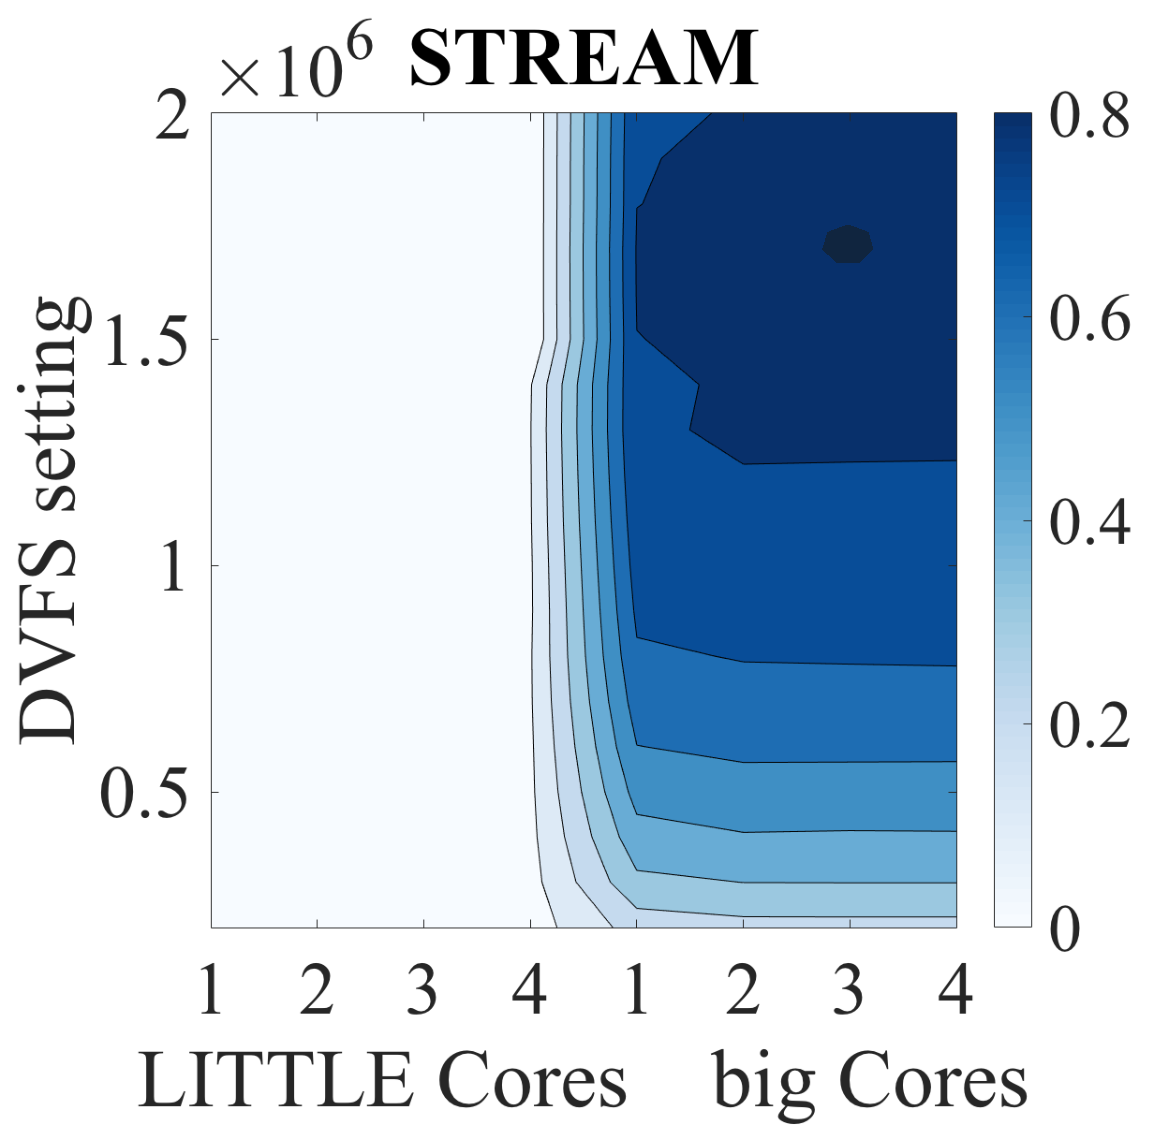
\includegraphics[width=.25\textwidth]{figures/STREAM-contour.pdf}
    \label{fig:STREAM_contour}
  }
  \subfloat[]
  {
    \begin{tikzpicture}
\begin{centering}

\definecolor{s1}{RGB}{228, 26, 28}
\definecolor{s2}{RGB}{55, 126, 184}
\definecolor{s3}{RGB}{77, 175, 74}
\definecolor{s4}{RGB}{152, 78, 163}
\definecolor{s5}{RGB}{255, 127, 0}

\begin{groupplot}[
    group style={
        group name=plots,
        group size=1 by 1,
        xlabels at=edge bottom,
        xticklabels at=edge bottom,
        vertical sep=5pt
    },
height=4.1cm,
width=0.45\columnwidth,
xmajorgrids,
ymajorgrids,
grid style={dashed},
xmax=20,
yticklabel pos=left,
enlargelimits=false,
tick align = outside,
tick style={white},
xticklabel shift={-5pt},
yticklabel shift={-5pt},
ylabel shift={-2pt},
ylabel style={align=center},
unbounded coords=jump,
]

\nextgroupplot[ylabel={\scriptsize Performance (Normalized)}, % Performance
xlabel={\footnotesize Iteration},
ymin=0,
ymax=1.5,
ytick={0.0,0.5,1.0,1.5},
yticklabels={,0.5,1.0,1.5},
legend entries={{\scriptsize $\mathsf{Performance Requirement}$},{\scriptsize $\mathsf{Learning}$},{\scriptsize $\mathsf{Adaptive Control}$},},
legend style={fill=none,draw=none,at={(0.5,1.4)},anchor=north,legend columns=1,line width=3pt},
]

\addplot[thick, solid, black] coordinates {(0,1) (20,1)};
\addplot[thick, solid, color=s4] table[x index=0,y index=1,col sep=space] {img/complexity-example-leo.txt};
\addplot[thick, solid, color=s5] table[x index=0,y index=1,col sep=space] {img/complexity-example-poet.txt};
\end{groupplot}
\end{centering}
\end{tikzpicture}
    \label{fig:STREAM_timeline}
  }
  \caption{(a) \texttt{STREAM} performance as a function of
    configuration.  (b) Managing \texttt{STREAM}'s performance:
    \emph{Learning} handles the complex configuration space, but
    \emph{control} oscillates.}
  \label{fig:learning-models1}
\end{figure}

We demonstrate how well learning handles complex resource interaction
for \texttt{STREAM} on an ARM big.LITTLE processor with four big,
high-performance cores and four LITTLE, energy efficient cores.  The
big cores support 19 clock speeds, while the LITTLE cores support 14.


\figref{fig:STREAM_contour} shows \texttt{STREAM}'s performance for
different resource configurations.  This memory-bound application has
complicated behavior: the LITTLE cores' memory hierarchy cannot
deliver the required performance.  The big cores' more powerful memory
system delivers much greater performance, but the peak occurs with 3
big cores.  Furthermore, at low clockspeeds, these 3 big cores cannot
saturate the memory bandwidth, while at high clockspeeds the
performance drops as the processor overheats, triggering thermal
management.  For \texttt{STREAM}, the peak speed occurs with 3 big
cores at 1.2 GHz, and it is not efficient to spend any time on the
LITTLE cores.  \texttt{STREAM}, however, does not have distinct
phases, so once a resource allocator finds the most energy efficient
configuration, it simply needs to maintain it.


\figref{fig:STREAM_timeline} shows 20 iterations of both learning
\cite{LEO} and adaptive control \cite{POET} allocating resources to
\texttt{STREAM}.  The x-axis shows iteration and the y-axis shows
performance normalized to the requirement.  The \emph{learning}
approach estimates \texttt{STREAM}'s performance and power for all
configurations and uses the lowest energy configuration that delivers
the required performance.  The \emph{adaptive controller} begins with
a generic notion of power/performance tradeoffs.  As the controller
runs, it measures performance and adjusts both the allocated resources
and its own parameters.  The adaptive controller dynamically adjusts
to non-linearities with a series of linear approximations; however,
inaccuracies in the relationship between resources and performance
cause oscillations that lead to performance violations.  This behavior
occurs because the controller's adaptive mechanisms cannot handle
STREAM's complexity, a known limitation of adaptive control systems
\cite{ControlWare,POET,ICSE2014}.  Hence, the \emph{learner}'s ability
to predict complex behavior is crucial.

\subsection{\emph{Controlling} Dynamics}

\begin{figure}
\centering
  \subfloat[]
  {
    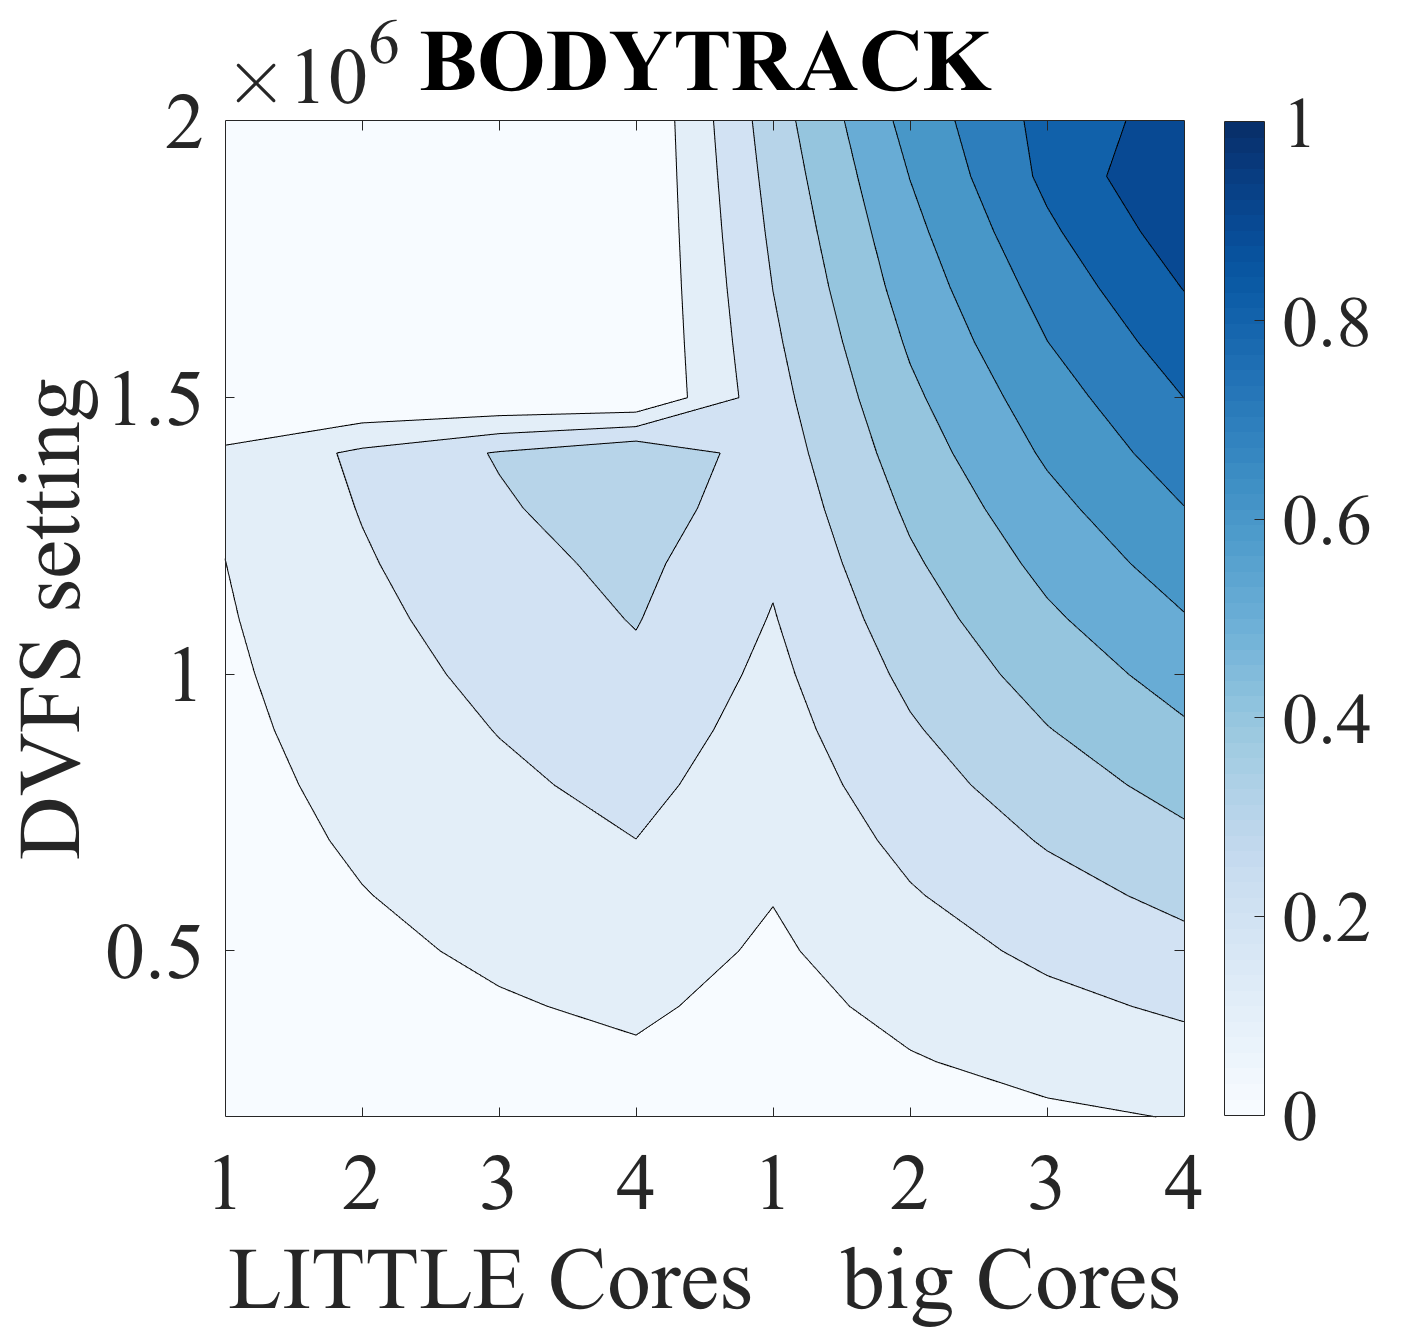
\includegraphics[width=.25\textwidth]{figures/BODYTRACK-contour.png}
    \label{fig:BODYTRACK_contour}
  }
  \subfloat[]
  {
    \begin{tikzpicture}
\begin{centering}

\definecolor{s1}{RGB}{228, 26, 28}
\definecolor{s2}{RGB}{55, 126, 184}
\definecolor{s3}{RGB}{77, 175, 74}
\definecolor{s4}{RGB}{152, 78, 163}
\definecolor{s5}{RGB}{255, 127, 0}

\begin{groupplot}[
    group style={
        group name=plots,
        group size=1 by 1,
        xlabels at=edge bottom,
        xticklabels at=edge bottom,
        vertical sep=5pt
    },
height=3.5cm,
width=0.45\columnwidth,
xmajorgrids,
ymajorgrids,
grid style={dashed},
xmin=0,
xmax=20,
yticklabel pos=left,
enlargelimits=false,
tick align = outside,
tick style={white},
xticklabel shift={-5pt},
yticklabel shift={-5pt},
ylabel shift={-2pt},
ylabel style={align=center},
unbounded coords=jump,
]

\nextgroupplot[ylabel={\scriptsize Performance (Normalized)}, % Performance
%xtick={0,500,1000,1500,2000,2500,3000,3500,4000,4500},
ytick={0.0,0.5,1.0,1.5,2.0},
yticklabels={,0.5,1.0,1.5,2.0},
xtick={90,95,100,105,110},
xticklabels={90,95,100,105,110},
%yticklabel style={font=\footnotesize},
xlabel={\footnotesize frame},
xmin=90,
xmax=110,
ymin=0,
ymax=1.5,
legend entries={{\scriptsize $\mathsf{Performance Requirement}$},{\scriptsize $\mathsf{Learning}$},{\scriptsize $\mathsf{Adaptive Control}$}},
legend style={fill=none,draw=none,at={(0.5,1.65)},anchor=north,legend columns=1,
line width=5pt},
]

\addplot[thick, solid, black] coordinates {(0,1) (399,1)};
\addplot[thick, solid, color=s4, mark=o] table[x index=0,y index=1,col sep=space] {img/dynamics-example-leo.txt};
\addplot[thick, solid, color=s5, mark=square] table[x index=0,y index=1,col sep=space] {img/dynamics-example-poet.txt};
\addplot[thick, dashed, black] coordinates {(99,0) (99,1.5)};
%\addplot[thick, dashed, black] coordinates {(130,0) (130, 2)};
\end{groupplot}
\end{centering}

\end{tikzpicture}

    \label{fig:BODYTRACK_timeline}    
  }
  \caption{(a) \texttt{bodytrack} performance as a function of
    configuration. (b) Managing \texttt{bodytrack}'s performance with
    another application: \emph{control} detects the change (at the
    vertical dashed line) and adjusts, but \emph{learning} cannot. }
  \label{fig:control}
\end{figure}


We now consider a dynamic environment.  We begin with
\texttt{bodytrack} running alone on the system.  Halfway through its
execution, we launch a second application---\texttt{STREAM}---on a
single big core, dynamically changing available resources.
\figref{fig:BODYTRACK_contour} shows \texttt{bodytrack}'s behavior.
It achieves the best performance on 4 big cores at the highest
clockspeed; the 4 LITTLE are more energy-efficient but slower.  For
\texttt{bodytrack}, the challenge is determining how to split time
between the LITTLE and big cores to conserve energy while still
meeting the performance requirements.

\figref{fig:BODYTRACK_timeline} shows the results of this experiment.
The vertical dashed line---at frame 99---represents when the second
application begins.  The figure clearly shows adaptive control's
benefits in this dynamic scenario.  When the second application
starts, the controller detects \texttt{bodytrack}'s performance
dip--rather than detecting the new application specifically---and it
changes resource allocation (increasing clockspeed and moving
bodytrack from 4 to 3 big cores).  The learning system however, does
not have any inherent mechanism to measure the change or adapt to the
altered performance.  While we could theoretically add feedback to the
learner and re-estimate the configuration space whenever the
environment changes, doing so is impractical due to high overhead for
learners capable of handling this complexity
\cite{Paragon,quasar,LEO}.


\subsection{Challenges of Interfacing Learning and Control}
The previous section motivate the first part of \SYSTEM{}: splitting
the resource allocation problem into prediction---which is handled by
learning---and dynamic management---which is handled by control. The
second part of \SYSTEM{}'s approach is the interface that combines the
two solutions.  This subsection demonstrates the importance of this
interface.

The controller's \emph{pole} is a particularly important control
parameter.  Control engineers tune the pole to trade response time for
noise sensitivity.  Traditionally, the data used to set the pole comes
from many observations of the controlled system and is considered
\emph{ground truth} \cite{Hellerstein2004a}.  \SYSTEM{}, however, must
tune the pole based on data from the learner, which may have noise
and/or errors.



\begin{wrapfigure}{r}{0.5\columnwidth} 
%\begin{figure}
%\centering
\begin{tikzpicture}
\begin{centering}

\definecolor{s1}{RGB}{228, 26, 28}
\definecolor{s2}{RGB}{55, 126, 184}
\definecolor{s3}{RGB}{77, 175, 74}
\definecolor{s4}{RGB}{152, 78, 163}
\definecolor{s5}{RGB}{255, 127, 0}

\begin{groupplot}[
    group style={
        group name=plots,
        group size=1 by 1,
        xlabels at=edge bottom,
        xticklabels at=edge bottom,
        vertical sep=5pt
    },
height=4.1cm,
width=0.45\columnwidth,
xmajorgrids,
ymajorgrids,
grid style={dashed},
xmin=0,
xmax=20,
yticklabel pos=left,
enlargelimits=false,
tick align = outside,
tick style={white},
xticklabel shift={-5pt},
yticklabel shift={-5pt},
ylabel shift={-2pt},
ylabel style={align=center},
unbounded coords=jump,
]

\nextgroupplot[ylabel={\scriptsize Performance (Normalized)}, % Performance
%xtick={0,500,1000,1500,2000,2500,3000,3500,4000,4500},
ytick={0.0,0.5,1.0,1.5,2.0},
yticklabels={,0.5,1.0,1.5,2.0},
xtick={90,95,100,105,110},
xticklabels={90,95,100,105,110},
%yticklabel style={font=\footnotesize},
xlabel={\footnotesize frame},
xmin=90,
xmax=110,
ymin=0,
ymax=1.5,
legend entries={{\scriptsize $\mathsf{Performance Requirement}$},{\scriptsize $\mathsf{Adaptive Control}$},{\scriptsize $\mathsf{Learning \& Control}$}},
legend style={fill=none,draw=none,at={(0.5,1.3)},anchor=north,legend columns=1,
line width=5pt},
]

\addplot[thick, solid, black] coordinates {(0,1) (399,1)};
\addplot[thick, solid, color=s5] table[x index=0,y index=1,col sep=space] {img/dynamics-example-poet.txt};
\addplot[thick, solid, color=s3] table[x index=0,y index=1,col sep=space] {img/dynamics-example-leopoetnp.txt};
\addplot[thick, dashed, black] coordinates {(99,0) (99,1.5)};
%\addplot[thick, dashed, black] coordinates {(130,0) (130, 2)};
\end{groupplot}
\end{centering}

\end{tikzpicture}

\caption{Comparison of carefully tuned and default poles.}
\label{fig:not-simple}
%\end{figure}
\end{wrapfigure}
To demonstrate the pole's importance when using a learned data, we
again control \texttt{bodytrack}, this time using the adaptive
controller from the previous subsection but instead of measuring
performance as a function of resource usage, we predict it, using the
learner from the first subsection.  We compare the results with a
carefully hand-tuned pole to those using the default pole provided by
the controller developers \cite{POET}.

\figref{fig:not-simple} shows the results.  The carefully tuned pole
converges because the pole accounts for possible errors in the learned
data. The default pole, however, oscillates around the performance
target, resulting in a number of missed deadlines.  Additionally, the
frames that exceed the desired performance waste energy because they
spend more time on the big, inefficient cores. The pole parameterizes
the system's \emph{inertia}---dictating how fast it should react to
environmental changes.  If the learner is noisy or inaccurate, the
controller should trust it less and move slowly. Rather than require
users with both computing and control knowledge to tune the pole,
\emph{\SYSTEM{} incorporates the learner's confidence interval and
  estimated variance to compute a pole that provides probabilistic
  convergence guarantees.}


